\documentclass{fast-nuces-bs}
%\documentclass{article}

\usepackage{blindtext}
\usepackage{mathptmx}% Times Roman font
\usepackage[T1]{fontenc}
\usepackage{lipsum} 
\usepackage{sectsty}
\usepackage{tikz-uml}
\usepackage{titlesec}
\usepackage{graphicx}
\usepackage{float}
\usepackage{tabularx}
\usepackage{booktabs}
\usepackage{longtable}
\usepackage{array}
\usepackage{multirow}
\usepackage{verbatim}


% Information about the Thesis 
% -----------------------------------------------------------------------------
%%%%%%%%%%%%%%%%%%%%%%%%%%%%%%%%%%%%%%%%%%%%%%%%%%%%%%%%%%%%%%%%%%%%%%%%%%%%%%%
\department{Department of Computer Science}
\faculty{Computer Science}
\degreeyear{2026}
\degreemonth{June}
\degreename{Computer Science}
\campuscity{Islamabad}
\authorone{muhammadaamirgulzar Kiyani}{muhammadaamirgulzar}
\authortwo{muhammadaamirgulzar}{muhammadaamirgulzar}
\authorthree{muhammadaamirgulzar}{muhammadaamirgulzar}
\supervisor{Sir Muhammad Aamir Gulzar}
\sessionduration{2022-2026}
\cosupervisor{Mr./ Ms./ Dr. Co-Supervisor Name}
\deanname{Dr. Dean Computing}
\directorname{Dr. Director of the Campus}
\hodname{Dr. Head of Computer Science Department}
\fypcoordinatorname{Name of FYP Coordinator}
\title{personalized-ai-storybook: LLM and Diffusion-Based Pipeline for Personalized Storybook Generation with Voice Narration and Evaluation}
%%%%%%%%%%%%%%%%%%%%%%%%%%%%%%%%%%%%%%%%%%%%%%%%%%%%%%%%%%%%%%%%%%%%%%%%%%%%%%%

%%%%%%%%%%%%%%%%%%%%%%%%%%%%%%%%%%%%%%%%%%%%%%%%%%%%%%%%%%%%%%%%%%%%%%%%%%%%%%
% Former document starts below this
\begin{document}

%\begin{acknowledgements}
%   The team would like to thank Sir Muhammad Aamir Gulzar for his continuous
%   guidance, feedback, and support throughout the FYP journey.
%\end{acknowledgements}

%\begin{abstract}
%personalized-ai-storybook is an AI-powered children's storybook generation platform that
%integrates local Large Language Models (Ollama/llama3.1:8b), Stable Diffusion
%image generation with IP-Adapter character consistency, Piper Text-to-Speech
%narration, OpenAI Whisper Speech-to-Text input, and a comprehensive evaluation
%framework (CLIP, Sentence Transformers, Flesch-Kincaid, InsightFace) into a
%cohesive, fully offline system. The system produces illustrated, narrated, and
%styled PDF storybooks through a multi-agent pipeline orchestrated by FastAPI,
%presented through an interactive open-book Next.js UI. All processing occurs
%locally, ensuring complete privacy for children's content creation.
%\end{abstract}

\chapter{Introduction}
\label{sec:introduction}

The rapid advancement of artificial intelligence technologies has opened unprecedented opportunities for creative content generation, fundamentally transforming how digital media is produced and consumed. This document presents \textbf{personalized-ai-storybook}, an innovative AI-powered platform that democratizes children's storybook creation through an integrated pipeline combining Large Language Models (LLMs) and diffusion-based image generation. Building upon the foundational work established in FYP-1, the current phase extends the system with six major enhancements: \textbf{Text-to-Speech (TTS) narration}, \textbf{Speech-to-Text (STT) voice input}, an \textbf{immersive styled open-book PDF export}, comprehensive \textbf{personalized and simple story enhancement pipelines}, a multi-metric \textbf{evaluation framework}, and significant \textbf{user interface improvements}.

The system architecture integrates a FastAPI backend orchestrating a multi-agent pipeline with a Next.js-based frontend, providing an intuitive open-book interface. All AI processing occurs locally using Ollama (llama3.1:8b-instruct-q4\_K\_M for story generation), Stable Diffusion 1.5 via WebUI API for image synthesis, Piper TTS for offline voice narration, and OpenAI Whisper for speech-to-text transcription—ensuring complete privacy and eliminating cloud dependencies.


\section{Existing Solutions}

The field of AI-powered storytelling has seen several commercial and research implementations, each with distinct approaches and limitations. Understanding these existing solutions provides context for the innovations introduced by personalized-ai-storybook.

\begin{table}[H]
\centering
\caption{Comparison of Existing Solutions}
\begin{tabular}{|c|p{5cm}|p{5cm}|}
\hline
\textbf{System Name} & \textbf{System Overview} & \textbf{System Limitations} \\ \hline
StoryBird & Cloud-based platform for creating illustrated children's books using pre-existing artwork. Provides templates and an artwork library for story composition. & Lacks AI-generated content, requires internet, limited character customization, subscription-based pricing, no TTS/STT, no character consistency across pages. \\ \hline
ChatGPT + DALL-E & General-purpose AI models that can generate stories and images separately through a conversational interface. & No integrated pipeline, no character consistency, cloud-dependent, no voice narration, requires manual prompt engineering per image, privacy concerns for children's data. \\ \hline
Canva Magic Write & Text generation tool with design capabilities for creating storybooks using templates and stock images. & Limited AI story generation depth, no character consistency, no TTS, not specialized for children's content, requires design expertise. \\ \hline
NovelAI & Subscription-based AI story and image generation service with customization options. & Cloud-dependent, requires subscription, complex interface, not optimized for children's content, no TTS narration, no offline mode. \\ \hline
\end{tabular}
\label{tab:system_comparison}
\end{table}


\section{Problem Statement}

The current landscape of digital storytelling presents several fundamental challenges that significantly limit effective content creation and user engagement. Existing AI-powered story generation platforms predominantly suffer from visual inconsistency, where character appearances vary dramatically across different pages of the same narrative, creating a disjointed reading experience that undermines story immersion. Many contemporary solutions require users to possess advanced prompt engineering skills to achieve quality outputs, establishing substantial barriers to entry for non-technical users, particularly children, parents, and educators who represent the primary target demographic for children's content.

The inherent separation between text generation and image creation processes in most platforms frequently results in misalignment, where generated illustrations fail to accurately represent the narrative context or scene descriptions. Furthermore, concerns regarding data privacy and the dependence on cloud-based services for AI processing create barriers for users seeking offline, privacy-preserving solutions for creating children's content. The complexity of existing creative tools and the cost of professional content creation services limit accessibility for families and educators with limited budgets.

Increasing reliance on passive digital media, especially among children, has reduced imagination and active participation in learning. Traditional educational content often lacks personalization, making it difficult to adapt to diverse student needs and cultural contexts. Existing systems lack voice-based interaction, meaning children who cannot type are excluded from the storytelling experience. There is also no mechanism to objectively evaluate the quality of generated stories and images — making it impossible to improve outputs systematically. Collectively, these challenges emphasize the need for a user-friendly, accessible, comprehensive, and consistent storytelling platform that maintains visual coherence, ensures data privacy, and delivers professional-quality illustrated and narrated storybooks without requiring technical expertise.


\section{Scope}

personalized-ai-storybook is designed as a comprehensive, offline, AI-powered storybook generation platform. The system supports the complete lifecycle of storybook creation — from voice or text input, through multi-agent story writing and image generation, to a narrated and exported illustrated PDF.

The full scope of this iteration encompasses:
\begin{itemize}
    \item \textbf{Text-to-Speech (TTS)}: Scene-by-scene audio narration using Piper TTS (offline ONNX models), with male/female voice selection and audio caching.
    \item \textbf{Speech-to-Text (STT)}: Voice story prompt submission using OpenAI Whisper (offline), with WAV preprocessing directly in Python (no ffmpeg dependency), resampled to 16kHz for Whisper compatibility.
    \item \textbf{Styled PDF Export}: Professional open-book layout PDF generation using ReportLab — dark leather cover, cream pages, red margin lines, notebook rulings, spine crease effects, and auto-scaling text.
    \item \textbf{Simple Story Enhancement}: Multi-agent pipeline (Director → Prompt → Writer → Reviewer → Editor) with background evaluation, content safety filtering, and dynamic genre/style/length customization.
    \item \textbf{Personalized Story Mode}: User-uploaded photo enables IP-Adapter (FaceID Plus v2) character consistency across all illustrations via Stable Diffusion WebUI API.
    \item \textbf{Evaluation Metrics}: Comprehensive multi-metric story quality assessment using CLIP (image-text alignment, visual consistency), Sentence Transformers (text coherence), Flesch-Kincaid (readability), InsightFace (character consistency in personalized mode), and a custom story structure validator.
    \item \textbf{UI Enhancements}: Interactive page-flipping open-book display, dark/light mode, character chatbot, idea workshop, audio playback controls per page, and voice input button.
\end{itemize}

The system does not support: real-time collaborative editing, cloud storage, mobile native apps (iOS/Android), or multi-language generation in this iteration.


\section{Modules}

The personalized-ai-storybook system is organized into six comprehensive modules, each responsible for specific aspects of the complete story generation, narration, and presentation pipeline.

\subsection{Large Language Model (LLM) + Multi-Agent Module}
This module manages story generation, enhancement, and structuring through a coordinated multi-agent pipeline. It handles the conversion of user prompts into structured stories and manages the multi-agent workflow for story creation.
\begin{enumerate}
    \item Local LLM integration via Ollama (llama3.1:8b-instruct-q4\_K\_M) for offline story generation.
    \item Director Agent for pipeline orchestration across all processing stages.
    \item Writer Agent for narrative generation, character development, and scene structuring.
    \item Reviewer Agent for quality assurance and age-appropriateness verification.
    \item Editor Agent for final polishing, formatting, and PDF export triggering.
    \item Prompt Agent for input validation, enhancement, and classification.
    \item Evaluation Agent (background) for multi-metric quality assessment of generated content.
    \item Idea Workshop Agent (LangChain-based) for interactive story ideation.
\end{enumerate}

\subsection{IP-Adapter + Stable Diffusion Module}
This module ensures character consistency and generates high-quality illustrations for each story page using Stable Diffusion 1.5 with IP-Adapter technology.
\begin{enumerate}
    \item Character consistency maintenance across all story illustrations using IP-Adapter FaceID Plus v2 via WebUI API.
    \item Stable Diffusion 1.5 with Realistic Vision checkpoint for high-quality image generation.
    \item Two-pass generation pipeline: initial txt2img synthesis followed by img2img enhancement.
    \item Genre and style-specific art generation (fantasy, cartoon, anime, realistic styles).
    \item Reference image processing for personalized story characters (user photo upload).
    \item GPU memory management (Ollama pause/resume during image generation).
\end{enumerate}

\subsection{Text-to-Speech (TTS) Module}
The TTS module provides scene-by-scene audio narration using local Piper TTS models.
\begin{enumerate}
    \item Page-by-page voice narration using Piper TTS (offline ONNX models, no internet required).
    \item Male (en\_US-ryan-medium) and female (en\_US-lessac-medium) voice selection.
    \item Audio caching — pre-generated WAV files reused to avoid redundant synthesis.
    \item Accessibility support for visually impaired users and young children.
    \item Audio synchronization with story page navigation in the frontend.
\end{enumerate}

\subsection{Speech-to-Text (STT) Module}
The STT module converts spoken user input into text story prompts using OpenAI Whisper.
\begin{enumerate}
    \item Offline speech-to-text using OpenAI Whisper (base model, no cloud needed).
    \item WAV file reading and resampling using Python built-in \texttt{wave} module and numpy (bypasses ffmpeg requirement).
    \item Automatic resampling to Whisper's required 16kHz sample rate.
    \item Stereo-to-mono conversion for broad microphone compatibility.
    \item Support for English language transcription with language auto-detection option.
\end{enumerate}

\subsection{PDF Rendering Module}
This module handles the generation of immersive, styled PDF storybooks using ReportLab.
\begin{enumerate}
    \item Styled PDF generation matching the open-book UI: dark leather cover, cream pages, spine crease effect.
    \item Professional book-cover page with story title, gold typography, and last scene image.
    \item Notebook-ruled text pages with red margin line and proportional auto-scaling font.
    \item Scene illustrations on the left page with white photo mat and drop shadow.
    \item Page number pill indicator on each scene spread.
    \item Georgia font family with fallback to Times-Roman for cross-system compatibility.
\end{enumerate}

\subsection{Context Management + UI Module}
This module orchestrates the entire workflow and manages user interface interactions.
\begin{enumerate}
    \item Next.js-based frontend with TypeScript for responsive, type-safe UI.
    \item Interactive open-book story display with page-by-page navigation.
    \item Audio playback controls (play/pause/voice selection) per story page.
    \item Voice input button for STT-based story prompt submission.
    \item Character chatbot powered by story context.
    \item Theme toggle (light/dark mode) with context-based state management.
    \item JWT-based authentication and PostgreSQL database integration.
    \item Genre, style, and length customization dropdowns.
\end{enumerate}


\section{Work Division}

The project responsibilities are distributed among team members based on their expertise and the modular architecture of the system. This FYP-2 phase adds new responsibilities reflecting the implemented features.

\clearpage

\begin{table}[H]
\centering
\caption{Work Division Table -- FYP-2}
\resizebox{\textwidth}{!}{%
\begin{tabular}{|p{0.25\textwidth}|p{0.15\textwidth}|p{0.60\textwidth}|}
\hline
\textbf{Name} & \textbf{Registration} & \textbf{Responsibility / Module / Feature} \\ \hline
muhammadaamirgulzar Kiyani & muhammadaamirgulzar & \textbf{TTS \& STT Integration}: Piper TTS implementation (offline ONNX, WAV generation, caching, voice selection), OpenAI Whisper STT (ffmpeg-free WAV reader, numpy resampler). \textbf{Evaluation Framework}: CLIP image-text alignment, visual consistency (CLIP), text coherence (Sentence Transformers), readability (Flesch-Kincaid), InsightFace character consistency for personalized mode, story structure validation, weighted overall score. \textbf{Personalized Story Mode}: IP-Adapter FaceID Plus v2, WebUI API integration, GPU memory management (Ollama pause/resume), LoRA verification. \textbf{Testing}: White-box unit tests (35 tests, 90\%+ average coverage), test infrastructure and coverage reporting. \textbf{Deployment}: Backend server configuration (FastAPI/Uvicorn), Ollama model setup, Stable Diffusion WebUI configuration, Python environment and dependency management. \\ \hline
muhammadaamirgulzar & muhammadaamirgulzar & \textbf{Styled PDF Export}: Full open-book layout PDF (leather cover, cream pages, spine crease, red margin, notebook ruling, auto-scaling font, Georgia typography, photo mat, drop shadow, page pill indicator). \textbf{UI Enhancement}: Simple vs.\ Personalized mode UI tabs, genre/style/length dropdowns, smooth page-flip transitions, loading animations. \textbf{Writer Agent}: Story generation pipeline, Stable Diffusion 1.5 setup, two-pass image generation (txt2img + img2img), illustration generation with style-specific prompts. \textbf{Deployment}: Frontend deployment (Next.js build configuration, static asset serving), PDF export pipeline setup, ReportLab font and asset path configuration for target environment. \\ \hline
muhammadaamirgulzar & muhammadaamirgulzar & \textbf{Full Pipeline Integration}: Connecting TTS/STT endpoints with frontend, audio playback UI (per-page controls, voice switcher), voice input button, character chatbot (story-context-powered), idea workshop interactive flow. \textbf{Backend API}: FastAPI endpoint management for TTS, STT, evaluation, story generation, and chat. \textbf{Simple Story Enhancement}: Prompt Agent, content safety filtering, multi-agent coordination. \textbf{Testing}: Black-box test cases (68 cases: equivalence partitioning, boundary value analysis, functional tests). \textbf{Deployment}: End-to-end system integration and deployment coordination, PostgreSQL database setup and migration, CORS and middleware configuration, cross-module bug-fixing and environment compatibility testing. \\ \hline
\end{tabular}%
}
\label{tab:work_division}
\end{table}

\chapter{Project Requirements}
\label{sec:requirements}

This chapter provides a comprehensive specification of the functional and non-functional requirements for the personalized-ai-storybook system as implemented in FYP-2. The requirements reflect the complete system including all FYP-2 additions: TTS, STT, styled PDF export, personalized and simple story enhancement, evaluation metrics, and UI improvements.

\section{Use-case Analysis}

The personalized-ai-storybook platform supports comprehensive operational workflows encompassing story generation, audio narration, voice input, personalized character rendering, interactive chat, idea workshop, and quality evaluation.

\subsection{Use-Case: Generate Story from Text Prompt (UC1)}
\textbf{Primary Actor}: Registered User \\
\textbf{Precondition}: User is authenticated and on the story generation page. \\
\textbf{Main Flow}:
\begin{enumerate}
    \item User selects ``Simple'' mode, enters a text prompt, and chooses genre/style/length.
    \item System validates and enhances the prompt via Prompt Agent.
    \item Director Agent orchestrates Writer → Reviewer → Editor pipeline.
    \item System generates illustrated scenes and exports a styled PDF.
    \item Story is displayed in the open-book UI with audio controls.
\end{enumerate}
\textbf{Postcondition}: Story is stored in the database; PDF is saved in \texttt{generated/exports/}.

\subsection{Use-Case: Generate Story from Voice Input (UC2)}
\textbf{Primary Actor}: Registered User \\
\textbf{Precondition}: User is on the story generation page; microphone is accessible. \\
\textbf{Main Flow}:
\begin{enumerate}
    \item User clicks the voice input button and speaks the story prompt.
    \item System records audio, sends WAV to \texttt{/api/stt} endpoint.
    \item Whisper STT transcribes speech to text.
    \item Transcribed text is pre-filled in the prompt field.
    \item User confirms and story generation proceeds as in UC1.
\end{enumerate}

\subsection{Use-Case: Listen to Story Narration (UC3)}
\textbf{Primary Actor}: Registered User \\
\textbf{Precondition}: Story has been generated and displayed. \\
\textbf{Main Flow}:
\begin{enumerate}
    \item User selects voice (male/female) from the audio control panel.
    \item User clicks ``Play'' for the current page.
    \item System calls \texttt{/api/tts} to generate/retrieve cached WAV audio.
    \item Audio plays through the browser; user can pause or switch pages.
\end{enumerate}

\subsection{Use-Case: Generate Personalized Story (UC4)}
\textbf{Primary Actor}: Registered User \\
\textbf{Precondition}: User selects ``Personalized'' mode and uploads a reference photo. \\
\textbf{Main Flow}:
\begin{enumerate}
    \item User uploads a photo in the personalized mode panel.
    \item System processes photo through IP-Adapter FaceID Plus v2.
    \item Story is generated; all illustrations maintain facial likeness using WebUI API.
    \item Personalized story is displayed and exported.
\end{enumerate}

\subsection{Use-Case: View Evaluation Metrics (UC5)}
\textbf{Primary Actor}: Registered User \\
\textbf{Precondition}: Story has been generated; evaluation has run in the background. \\
\textbf{Main Flow}:
\begin{enumerate}
    \item Evaluation Agent runs asynchronously after story generation.
    \item Computes: image-text alignment, visual consistency, text coherence, readability, story structure.
    \item Results stored in \texttt{generated/evaluations/} as JSON.
    \item User can view quality metrics in the story details panel.
\end{enumerate}

\subsection{Use-Case: Chat with Story Character (UC6)}
\textbf{Primary Actor}: Registered User \\
\textbf{Main Flow}: User selects a character from the story; types a message; Chatbot Agent responds in character using story context.

\subsection{Use-Case: Idea Workshop (UC7)}
\textbf{Primary Actor}: Registered User \\
\textbf{Main Flow}: User starts a workshop session; the LangChain-based Idea Workshop Agent collects story requirements through multi-turn conversation; confirms all fields; generates the story.

\subsection{Use-Case: Export Story to PDF (UC8)}
\textbf{Primary Actor}: Registered User \\
\textbf{Main Flow}: Upon story completion, system automatically calls the EditorAgent PDF export; the styled PDF with leather cover and notebook-ruled text pages is saved and available for download.


\section{Functional Requirements}

\subsection{Multi-Agent Story Generation Module}
\begin{enumerate}
    \item \textbf{FR1.1}: The system shall accept user prompts ranging from 5 to 500 characters for story generation.
    \item \textbf{FR1.2}: The Prompt Agent shall validate and classify prompts as normal, detailed, invalid, or nonsense.
    \item \textbf{FR1.3}: The Prompt Agent shall enhance simple prompts by adding contextual details.
    \item \textbf{FR1.4}: The Director Agent shall orchestrate the sequential execution of Prompt, Writer, Reviewer, and Editor agents.
    \item \textbf{FR1.5}: The Writer Agent shall generate structured stories using Ollama LLM (llama3.1:8b-instruct-q4\_K\_M) with title, setting, characters, and exactly 3 scenes.
    \item \textbf{FR1.6}: The Writer Agent shall retry up to 2 times if JSON parsing fails.
    \item \textbf{FR1.7}: The Reviewer Agent shall validate content for coherence, age-appropriateness, and educational value.
    \item \textbf{FR1.8}: The Editor Agent shall finalize the story and trigger PDF export.
    \item \textbf{FR1.9}: The Evaluation Agent shall run asynchronously in the background after generation.
    \item \textbf{FR1.10}: The system shall output stories in comprehensive JSON format with metadata and scene image paths.
    \item \textbf{FR1.11}: The Content Safety module shall block explicit, violent, or inappropriate prompts and image descriptions.
    \item \textbf{FR1.12}: The Idea Workshop Agent shall collect story requirements through multi-turn LangChain conversation before generating.
\end{enumerate}

\subsection{Image Generation Module}
\begin{enumerate}
    \item \textbf{FR2.1}: The Image Agent shall generate illustrations for each scene using Stable Diffusion 1.5 with Realistic Vision checkpoint.
    \item \textbf{FR2.2}: The system shall employ a two-pass generation: txt2img at 512$\times$512 followed by img2img at 768$\times$768.
    \item \textbf{FR2.3}: The system shall use DPMSolver++ 2M Karras scheduler for optimized sampling.
    \item \textbf{FR2.4}: In Personalized mode, the system shall apply IP-Adapter FaceID Plus v2 embeddings via WebUI API.
    \item \textbf{FR2.5}: The system shall pause/resume Ollama service during image generation to manage GPU memory.
    \item \textbf{FR2.6}: The system shall continue story generation with text only if image generation fails.
\end{enumerate}

\subsection{Text-to-Speech Module}
\begin{enumerate}
    \item \textbf{FR3.1}: The system shall generate WAV audio narration for each story scene using Piper TTS (offline ONNX models).
    \item \textbf{FR3.2}: The system shall support male (en\_US-ryan-medium) and female (en\_US-lessac-medium) voice options.
    \item \textbf{FR3.3}: The system shall cache generated audio files to avoid redundant synthesis on re-request.
    \item \textbf{FR3.4}: TTS audio shall be served via static file routes accessible to the frontend.
    \item \textbf{FR3.5}: The system shall expose a \texttt{POST /api/tts} endpoint accepting story\_id, scene\_number, and voice parameters.
\end{enumerate}

\subsection{Speech-to-Text Module}
\begin{enumerate}
    \item \textbf{FR4.1}: The system shall transcribe WAV audio files to text using OpenAI Whisper (base model, offline).
    \item \textbf{FR4.2}: The system shall read WAV files using Python's built-in \texttt{wave} module without requiring ffmpeg.
    \item \textbf{FR4.3}: The system shall resample audio to 16kHz using numpy linear interpolation for Whisper compatibility.
    \item \textbf{FR4.4}: The system shall convert stereo recordings to mono automatically.
    \item \textbf{FR4.5}: The system shall expose a \texttt{POST /api/stt} endpoint accepting an audio file upload.
    \item \textbf{FR4.6}: The system shall return the transcribed text and detected language in the response.
\end{enumerate}

\subsection{PDF Rendering Module}
\begin{enumerate}
    \item \textbf{FR5.1}: The system shall generate a styled PDF storybook matching the open-book UI design.
    \item \textbf{FR5.2}: The PDF shall include a cover page with leather/cream layout, story title in gold typography, and last scene image.
    \item \textbf{FR5.3}: Each scene shall be rendered as a spread: illustration on the left with white photo mat; text on the right with red margin line and notebook rulings.
    \item \textbf{FR5.4}: Text shall auto-scale (14pt down to 10pt) to prevent overflow.
    \item \textbf{FR5.5}: The PDF shall use Georgia font with fallback to Times-Roman.
    \item \textbf{FR5.6}: The system shall use A4 landscape orientation with a leather-brown background frame.
    \item \textbf{FR5.7}: Each scene page shall include a page number pill indicator.
\end{enumerate}

\subsection{Evaluation Module}
\begin{enumerate}
    \item \textbf{FR6.1}: The Evaluation Agent shall assess image-text alignment using CLIP cosine similarity (OpenAI CLIP ViT-B/32).
    \item \textbf{FR6.2}: The system shall evaluate visual consistency across scene images using CLIP image embeddings.
    \item \textbf{FR6.3}: The system shall evaluate text coherence between consecutive scenes using Sentence Transformers.
    \item \textbf{FR6.4}: The system shall assess readability using Flesch-Kincaid grade level (target: grades 3--6 for ages 7--10).
    \item \textbf{FR6.5}: The system shall validate story structure (beginning, climax, ending) using a heuristic scorer.
    \item \textbf{FR6.6}: In Personalized mode, the system shall evaluate character face consistency using InsightFace embeddings.
    \item \textbf{FR6.7}: The system shall compute a weighted overall score (0--100) and save results as JSON.
\end{enumerate}

\subsection{User Interface and Frontend Module}
\begin{enumerate}
    \item \textbf{FR7.1}: The frontend shall provide a Next.js-based responsive open-book UI.
    \item \textbf{FR7.2}: The story display shall present a left page (illustration) and right page (story text) with page-flip navigation.
    \item \textbf{FR7.3}: Each page shall include audio controls (play/pause button, voice selector).
    \item \textbf{FR7.4}: The UI shall include a voice input button for speech-to-text story prompt submission.
    \item \textbf{FR7.5}: The system shall provide theme toggle for light/dark mode.
    \item \textbf{FR7.6}: The UI shall support genre, style, and length customization dropdowns.
    \item \textbf{FR7.7}: The UI shall display custom loading animations during story generation.
    \item \textbf{FR7.8}: Simple and Personalized mode tabs shall be clearly separated in the UI.
\end{enumerate}


\section{Non-Functional Requirements}

\subsection{Performance}
\begin{itemize}
    \item \textbf{PER-1}: Story text generation shall complete within 10--15 seconds on systems with 16GB RAM.
    \item \textbf{PER-2}: Image generation per scene shall complete within 35--45 seconds on GPU (NVIDIA GTX 1060 or equivalent).
    \item \textbf{PER-3}: TTS audio generation per scene shall complete within 2--5 seconds using Piper.
    \item \textbf{PER-4}: STT transcription shall complete within 3--8 seconds for a 15-second voice prompt.
    \item \textbf{PER-5}: Evaluation Agent shall run asynchronously and not block the story generation response.
    \item \textbf{PER-6}: PDF export shall complete within 3--5 seconds for a 3-scene story.
\end{itemize}

\subsection{Reliability}
\begin{itemize}
    \item \textbf{REL-1}: The Writer Agent shall successfully generate valid JSON for 90\% of reasonable prompts.
    \item \textbf{REL-2}: The system shall retry up to 2 times on JSON parsing failures.
    \item \textbf{REL-3}: The system shall deliver text-only stories when image generation fails (graceful degradation).
    \item \textbf{REL-4}: TTS shall return an empty string rather than crashing if Piper synthesis fails.
    \item \textbf{REL-5}: STT shall raise a descriptive exception rather than silently failing.
    \item \textbf{REL-6}: The Evaluation Agent shall handle missing images gracefully with default scores.
\end{itemize}

\subsection{Usability}
\begin{itemize}
    \item \textbf{USE-1}: Users with no technical background shall be able to generate a story within 3 interactions.
    \item \textbf{USE-2}: The UI shall provide clear visual feedback (loading spinner, progress messages) during all operations.
    \item \textbf{USE-3}: The system shall display user-friendly error messages when generation fails.
    \item \textbf{USE-4}: Voice input shall be accessible via a single button click without configuration.
    \item \textbf{USE-5}: Audio narration shall start within 1 second of the user clicking play (from cache).
\end{itemize}

\subsection{Security}
\begin{itemize}
    \item \textbf{SEC-1}: All AI processing shall occur locally without transmitting user data to external servers.
    \item \textbf{SEC-2}: User authentication shall use JWT tokens with bcrypt password hashing.
    \item \textbf{SEC-3}: User-uploaded reference photos shall not be stored permanently without user consent.
    \item \textbf{SEC-4}: The Content Safety module shall block inappropriate content before generation.
\end{itemize}

\subsection{Maintainability}
\begin{itemize}
    \item \textbf{MNT-1}: Each agent module shall be independently implementable and testable.
    \item \textbf{MNT-2}: TTS and STT managers shall use a singleton pattern for resource efficiency.
    \item \textbf{MNT-3}: All evaluation scores shall be in a unified 0--100 integer scale for easy interpretation.
    \item \textbf{MNT-4}: The codebase shall include inline comments and docstrings for all key functions.
\end{itemize}

\subsection{Portability}
\begin{itemize}
    \item \textbf{PORT-1}: The system shall operate on Windows 10/11 systems (primary development platform).
    \item \textbf{PORT-2}: The STT module shall not require ffmpeg installation (pure Python WAV reader).
    \item \textbf{PORT-3}: The TTS module shall use offline ONNX Piper models, requiring no internet.
    \item \textbf{PORT-4}: The system shall function on both CPU-only and GPU-enabled hardware.
\end{itemize}

\chapter{System Overview}
\label{sec:system_overview}

This chapter provides a comprehensive description of the personalized-ai-storybook system architecture, design patterns, and technical implementation for the FYP-2 phase. The system integrates six major new modules (TTS, STT, styled PDF, evaluation, and UI enhancements) into the existing multi-agent pipeline.

\section{Architectural Design}

personalized-ai-storybook employs a layered architecture pattern to achieve modularity, maintainability, and clarity of responsibility. The architecture consists of six distinct layers, each with well-defined responsibilities and clear interfaces for inter-layer communication.

\subsection{Architecture Layers}

\textbf{1. Presentation Layer (Frontend)} \\
The topmost layer handles all user interactions and visual presentation. It comprises the Next.js-based UI with TypeScript, including:
\begin{itemize}
    \item Landing page with mode selection (Simple vs.\ Personalized)
    \item Multi-modal input interface: text prompt field, voice input button (STT), and file upload (personalized photo)
    \item Open-book story display: illustration left page, story text right page, page-flip navigation
    \item Per-page audio controls (play/pause, voice selector) for TTS playback
    \item Character Chatbot and Idea Workshop panels
    \item Theme toggle (light/dark mode) and customization dropdowns (genre, style, length)
\end{itemize}

\textbf{2. Application Layer (Backend API)} \\
FastAPI (main.py) acts as the entry point for all backend operations:
\begin{itemize}
    \item \texttt{POST /api/generate} — Story generation (simple or personalized)
    \item \texttt{POST /api/tts} — Audio narration generation/retrieval
    \item \texttt{POST /api/stt} — Speech-to-text transcription
    \item \texttt{POST /api/chat} — Character chatbot interaction
    \item \texttt{POST /api/workshop/session} and \texttt{/message} — Idea workshop
    \item \texttt{GET /api/stories} — User story history
    \item \texttt{GET /device} — Hardware detection (GPU/CPU)
\end{itemize}

\textbf{3. Business Logic Layer (Multi-Agent System)} \\
This layer contains the core domain logic and specialized agent implementations:
\begin{itemize}
    \item \textbf{PromptAgent} — Input validation, enhancement, classification
    \item \textbf{DirectorAgent} — Orchestrates the Writer → Reviewer → Editor pipeline
    \item \textbf{WriterAgent} — Story generation via Ollama LLM
    \item \textbf{ReviewerAgent} — Quality assurance and age-appropriateness
    \item \textbf{EditorAgent} — Final polish and PDF export (ReportLab open-book layout)
    \item \textbf{ImageAgent} — Standard Stable Diffusion image generation
    \item \textbf{PersonalizedImageAgent} — IP-Adapter FaceID Plus v2 via WebUI API
    \item \textbf{ChatbotAgent} — Story-context-aware character conversations
    \item \textbf{IdeaWorkshopAgent} — LangChain-based multi-turn story ideation
    \item \textbf{EvaluationAgent} — Asynchronous quality metrics computation
\end{itemize}

\textbf{4. AI/ML Layer (Model Inference)} \\
The most computationally intensive layer:
\begin{itemize}
    \item \textbf{Ollama} — Local LLM inference (llama3.1:8b-instruct-q4\_K\_M, mistral-nemo:12b for workshop)
    \item \textbf{Stable Diffusion WebUI} — Image generation with IP-Adapter; txt2img + img2img pipeline
    \item \textbf{Piper TTS} — Offline ONNX text-to-speech synthesis
    \item \textbf{OpenAI Whisper} — Offline speech-to-text transcription
    \item \textbf{CLIP} (ViT-B/32) — Image-text alignment and visual consistency evaluation
    \item \textbf{Sentence Transformers} — Text coherence evaluation
    \item \textbf{InsightFace} — Character face consistency evaluation (personalized mode)
    \item \textbf{PyTorch} — Tensor operations and device management (CUDA/CPU)
\end{itemize}

\textbf{5. Data Layer (Hybrid Storage)} \\
\begin{itemize}
    \item \textbf{PostgreSQL} (SQLAlchemy ORM) — Users, stories, chat sessions, workshop sessions and messages
    \item \textbf{File System} — \texttt{generated/images/}, \texttt{generated/audio/}, \texttt{generated/exports/}, \texttt{generated/evaluations/}, \texttt{generated/stories/}
\end{itemize}

\textbf{6. Infrastructure Layer} \\
\begin{itemize}
    \item OllamaManager — GPU memory management (pause/resume Ollama during image generation)
    \item ContentSafety — Blocked/warning keyword filtering for prompts and image descriptions
    \item EvaluationManager — Singleton evaluation orchestrator with lazy model loading
    \item TTSManager — Singleton Piper TTS with audio caching
    \item WhisperSTTManager — Singleton Whisper with ffmpeg-free WAV reader
\end{itemize}

\subsection{Key Design Patterns}

\textbf{Facade Pattern}: The \texttt{StoryAgent} class provides a simplified interface to the complex multi-agent pipeline orchestrated by the \texttt{DirectorAgent}. \\
\textbf{Pipeline Pattern}: Story generation follows a sequential pipeline — Prompt Agent → Writer Agent → Reviewer Agent → Editor Agent — where each agent transforms and passes data to the next stage. \\
\textbf{Singleton Pattern}: \texttt{TTSManager}, \texttt{WhisperSTTManager}, and \texttt{EvaluationManager} are all singletons, ensuring models are loaded once and reused across requests. \\
\textbf{Strategy Pattern}: The \texttt{generate\_images} flag and \texttt{use\_personalized\_images} flag act as strategy selectors, choosing between text-only, standard, or personalized image generation. \\
\textbf{Observer Pattern (Async)}: The \texttt{EvaluationAgent} is triggered asynchronously after story completion, observing the completed story without blocking the main response.


\section{Design Models}

This section presents detailed design models capturing the system's behavior, structure, and data flow.

\subsection{Use Case Diagram}

The use case diagram illustrates the primary interactions between two actor types --- the \textbf{Registered User} and the \textbf{System (Background)} --- and the eight core use cases of personalized-ai-storybook FYP-2.

\begin{figure}[H]
    \centering
    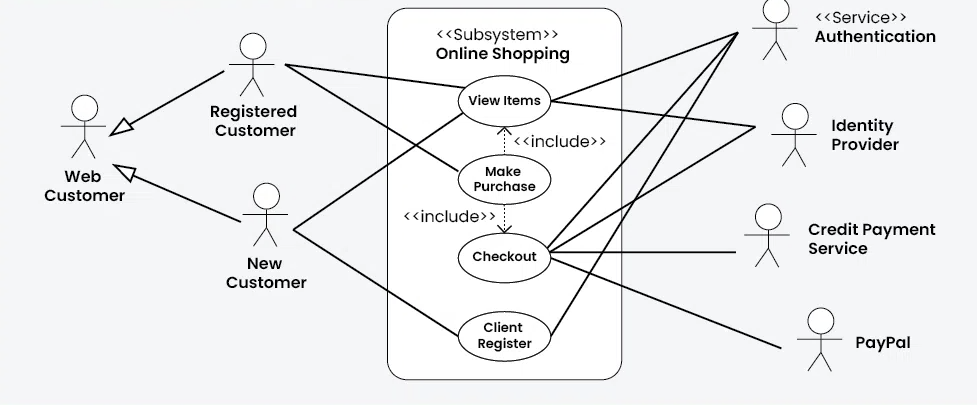
\includegraphics[width=\textwidth]{images/usecaseexample.png}
    \caption{Use Case Diagram -- personalized-ai-storybook FYP-2 (see diagram file: \texttt{diagrams/use\_case.puml})}
    \label{fig:usecase}
\end{figure}

\textbf{Actors and Use Cases:}
\begin{itemize}
    \item \textbf{Registered User}: Generate Story from Text (UC1), Generate Story from Voice (UC2), Listen to Narration (UC3), Generate Personalized Story (UC4), View Evaluation Metrics (UC5), Chat with Character (UC6), Idea Workshop (UC7), Export to PDF (UC8).
    \item \textbf{System (Background)}: Run Evaluation Agent (triggered automatically after generation).
\end{itemize}

\subsection{Activity Diagram}

The activity diagram illustrates the complete story generation workflow from user input to final output, covering both Simple and Personalized modes.

\textbf{Key Activities}:
\begin{enumerate}
    \item User selects mode (Simple / Personalized) and provides input (text or voice).
    \item [STT path] Audio is transcribed by Whisper; text is returned.
    \item Prompt Agent validates and enhances prompt; content safety check.
    \item Director Agent orchestrates: Writer → Reviewer → Editor.
    \item [Personalized path] IP-Adapter photo is processed; Ollama paused for GPU.
    \item Image Agent generates scene illustrations (txt2img → img2img).
    \item Editor Agent exports styled PDF (leather cover, notebook pages).
    \item Evaluation Agent runs asynchronously; results stored.
    \item Story displayed in open-book UI with TTS controls.
\end{enumerate}

\subsection{Data Flow Diagram}

The DFD models the data flow through the personalized-ai-storybook system across three levels.

\subsubsection{Context Diagram (DFD Level 0)}

The context diagram shows the system boundary and external entities:

\begin{itemize}
    \item \textbf{External Entities}: User (provides prompts, voice audio, reference photos; receives stories, audio, PDFs), Ollama Server (LLM inference), Stable Diffusion WebUI (image generation), PostgreSQL Database (data persistence).
    \item \textbf{Central Process}: personalized-ai-storybook System (receives inputs, produces storybook outputs).
    \item \textbf{Data Flows}: User Prompt → System; Voice Audio → System; Reference Photo → System; Story JSON ← System; Audio WAV ← System; PDF ← System.
\end{itemize}

\begin{figure}[H]
    \centering
    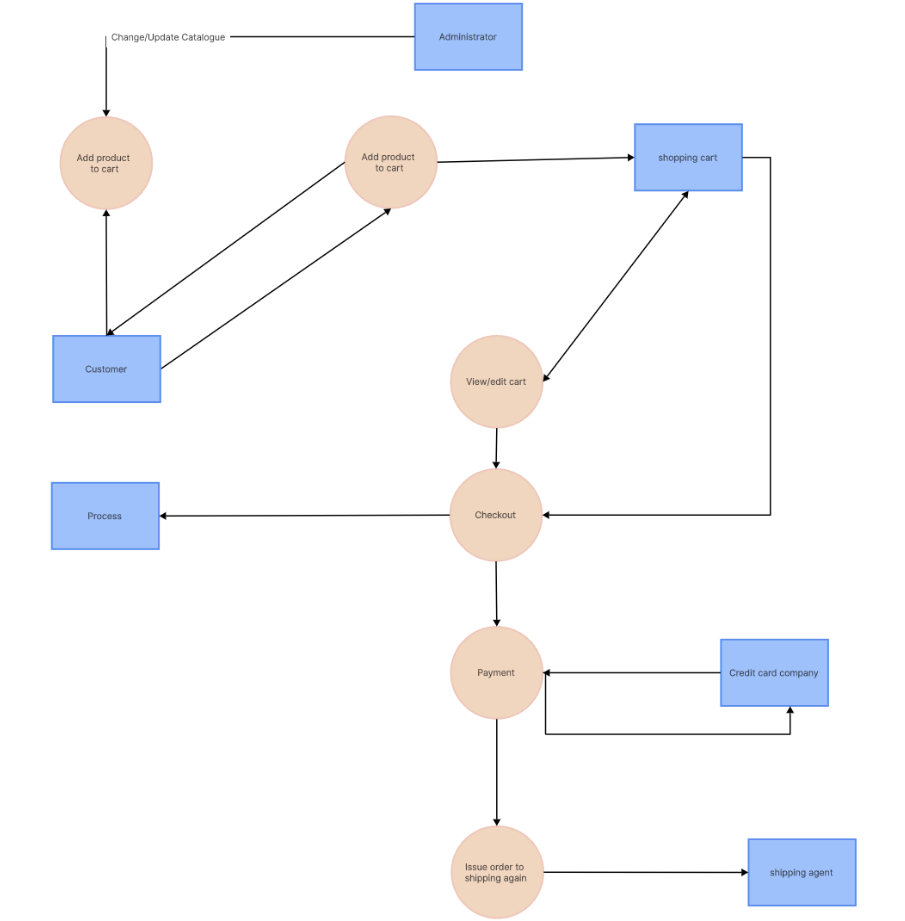
\includegraphics[width=0.85\textwidth]{images/dfd.png}
    \caption{Context Diagram (DFD Level 0) -- personalized-ai-storybook (see: \texttt{diagrams/dfd\_context.puml})}
    \label{fig:dfd_context}
\end{figure}

\subsubsection{Level 1 DFD}

The Level 1 DFD decomposes the system into six main processes:

\begin{enumerate}
    \item \textbf{1.0 Process User Input} — Receives text/voice, validates, converts STT; outputs: enhanced prompt.
    \item \textbf{2.0 Generate Story Text} — Multi-agent pipeline (Writer/Reviewer/Editor); reads/writes STORIES store; outputs: story JSON.
    \item \textbf{3.0 Generate Illustrations} — Receives scene descriptions; writes IMAGES store; outputs: image paths.
    \item \textbf{4.0 Synthesize Audio} — Receives scene text; reads/writes AUDIO store; outputs: WAV paths.
    \item \textbf{5.0 Export PDF} — Receives story+images; writes EXPORTS store; outputs: PDF path.
    \item \textbf{6.0 Evaluate Quality} — Receives story+images; writes EVALUATIONS store; outputs: metrics JSON.
\end{enumerate}

\subsubsection{Level 2 DFD -- Story Generation (Process 2.0)}

Process 2.0 expands into:
\begin{itemize}
    \item \textbf{2.1 Validate \& Enhance Prompt} (Prompt Agent): receives raw prompt → outputs enhanced prompt.
    \item \textbf{2.2 Generate Story Draft} (Writer Agent): calls Ollama; retries on JSON failure; outputs story draft.
    \item \textbf{2.3 Review Story} (Reviewer Agent): checks coherence/age-appropriateness; outputs reviewed story.
    \item \textbf{2.4 Edit \& Finalize} (Editor Agent): polishes text; saves to STORIES store; triggers PDF export.
\end{itemize}

\subsection{Class Diagram}

The class diagram illustrates the object-oriented structure, showing the key agent classes, their attributes, methods, and relationships. See the diagram files for the full PlantUML source (\texttt{diagrams/class\_diagram.puml}).

\textbf{Key Classes and Relationships}:
\begin{itemize}
    \item \textbf{DirectorAgent} (orchestrator) → aggregates WriterAgent, ReviewerAgent, EditorAgent, ImageAgent.
    \item \textbf{StoryAgent} (facade) → delegates to DirectorAgent.
    \item \textbf{PersonalizedImageAgent} (extends ImageAgent) → uses WebUI API with IP-Adapter.
    \item \textbf{ChatbotAgent} — depends on Story (context); associated with ChatConversation.
    \item \textbf{IdeaWorkshopAgent} — aggregates WorkshopSession and WorkshopMessage.
    \item \textbf{TTSManager} (singleton) — generates/caches WAV files.
    \item \textbf{WhisperSTTManager} (singleton) — transcribes WAV audio.
    \item \textbf{EvaluationManager} (singleton) — orchestrates all evaluation metrics.

\end{itemize}

\subsection{Sequence Diagram: TTS Audio Narration}

This sequence diagram illustrates the Text-to-Speech audio generation flow:
\begin{enumerate}
    \item User clicks ``Play'' on story page; frontend sends \texttt{POST /api/tts} with \{story\_id, scene\_number, voice\}.
    \item FastAPI routes request to \texttt{TTSManager.generate\_audio()}.
    \item TTSManager checks audio cache; if exists, returns cached relative path.
    \item If not cached: writes scene text to temp file; invokes Piper TTS subprocess via PowerShell.
    \item WAV file saved to \texttt{generated/audio/}; path returned to frontend.
    \item Frontend loads audio from static file route and plays through browser audio element.
\end{enumerate}

\subsection{Sequence Diagram: STT Voice Input}

\begin{enumerate}
    \item User clicks voice input button; browser records audio and sends WAV to \texttt{POST /api/stt}.
    \item FastAPI saves WAV to temp file; calls \texttt{WhisperSTTManager.transcribe\_audio()}.
    \item STT manager reads WAV using built-in \texttt{wave} module (no ffmpeg); converts to float32 numpy array.
    \item Audio resampled from original rate to 16kHz using numpy linear interpolation.
    \item Whisper model transcribes audio; returns \{text, language\}.
    \item FastAPI returns transcribed text to frontend; pre-filled in prompt field.
\end{enumerate}

\subsection{State Transition Diagram}

The state diagram models the lifecycle of a Story object within the system:

\textbf{States}: IDLE → PROMPT\_RECEIVED → VALIDATING → GENERATING\_TEXT → REVIEWING → EDITING → GENERATING\_IMAGES (optional) → EXPORTING\_PDF → EVALUATING (background) → COMPLETED → NARRATING (on user demand) \\
\textbf{Key Transitions}:
\begin{itemize}
    \item IDLE → PROMPT\_RECEIVED: User submits prompt (text or via STT).
    \item GENERATING\_IMAGES → EXPORTING\_PDF: Image generation completes (or times out).
    \item COMPLETED → NARRATING: User clicks play on any scene page.
    \item Any state → ERROR: On unrecoverable exception; system logs and returns error response.
\end{itemize}


\section{Data Design}

The system uses a hybrid data storage approach: structured PostgreSQL for user/session data and file-based storage for generated content.

\subsection{Database Schema}

The PostgreSQL database consists of 7 tables managed via SQLAlchemy ORM:

\begin{itemize}
    \item \textbf{Users}: id, username, email, hashed\_password, created\_at.
    \item \textbf{Stories}: id, user\_id (FK), title, story\_json, pdf\_path, mode, created\_at.
    \item \textbf{ChatConversations}: id, story\_id (FK), character\_name, created\_at.
    \item \textbf{ChatMessages}: id, conversation\_id (FK), role, content, timestamp.
    \item \textbf{WorkshopSessions}: id, user\_id (FK), mode, status, created\_at.
    \item \textbf{WorkshopMessages}: id, session\_id (FK), role, content, metadata, timestamp.
    \item \textbf{WorkshopStories}: id, session\_id (FK), story\_json, version, created\_at.
\end{itemize}

\subsection{File System Storage}

Generated content is organized in dedicated directories under \texttt{generated/}:
\begin{itemize}
    \item \texttt{images/} — PNG scene illustrations (timestamped filenames).
    \item \texttt{audio/} — WAV narration files (story\_\{id\}\_scene\_\{n\}\_\{voice\}.wav).
    \item \texttt{exports/} — Styled PDF storybooks.
    \item \texttt{evaluations/} — JSON quality metrics reports.
    \item \texttt{stories/} — Final JSON story objects.
    \item \texttt{drafts/}, \texttt{prompts/}, \texttt{reviews/}, \texttt{edits/} — Agent intermediate outputs.
\end{itemize}

\subsection{JSON Story Structure}

Stories are represented in a standardized JSON schema validated by Pydantic:
\begin{itemize}
    \item \texttt{title}: String story title.
    \item \texttt{setting}: String describing the story world.
    \item \texttt{characters}: Array of character names.
    \item \texttt{scenes}: Array of \{scene\_number, text, image\_description, image\_path, image\_url\}.
    \item \texttt{meta}: Optional metadata (genre, style, prompt\_type, enhanced\_prompt, mode).
    \item \texttt{mode}: ``simple'' | ``personalized''.
    \item \texttt{finalized}: Boolean; true after EditorAgent completes.
\end{itemize}


\section{Domain Model}

The domain model represents the core business entities and their relationships in personalized-ai-storybook FYP-2:

\begin{itemize}
    \item \textbf{User}: Authenticated platform user; creates Stories; participates in WorkshopSessions.
    \item \textbf{Story}: A complete generated storybook with title, setting, characters, scenes, metadata, mode, and optional audio paths.
    \item \textbf{Scene}: Individual page of a story with text, image description, image path, and audio path.
    \item \textbf{Agent (Abstract)}: Base for PromptAgent, WriterAgent, ReviewerAgent, EditorAgent, ImageAgent, PersonalizedImageAgent, ChatbotAgent, IdeaWorkshopAgent, EvaluationAgent.
    \item \textbf{TTSManager}: Generates and caches WAV narration per scene.
    \item \textbf{WhisperSTTManager}: Transcribes user voice input.
    \item \textbf{EvaluationReport}: Quality assessment result with per-metric scores and overall weighted score.
    \item \textbf{WorkshopSession}: Interactive story ideation session with conversation history.
    \item \textbf{ChatConversation}: Character chatbot session linked to a specific Story.
\end{itemize}

\chapter{Implementation and Testing}
\label{sec:implementation}

This chapter documents the technical implementation details, algorithms, external dependencies, and testing strategies for the personalized-ai-storybook FYP-2 system. The implementation demonstrates practical application of AI technologies across six new modules (TTS, STT, styled PDF, evaluation, personalized story, and UI enhancements).

\section{Algorithm Design}

\subsection{Multi-Agent Story Generation Pipeline (Enhanced)}

The core story generation algorithm remains a sequential multi-agent pipeline, extended with background evaluation, TTS triggering, and STT preprocessing.

\begin{verbatim}
ALGORITHM: Enhanced Multi-Agent Story Generation
INPUT:  user_prompt (string | audio), generate_images (bool),
        use_personalized_images (bool), user_photo (image | None),
        voice (string), genre, style, length
OUTPUT: complete_story (JSON), pdf_path (string), status

BEGIN
  1. IF audio_input THEN
       audio = STTManager.transcribe_audio(audio_file)
       user_prompt = audio.text
  
  2. PromptAgent.process_prompt(user_prompt)
     - Validate length [5-500 chars]
     - Classify: normal | detailed | invalid | nonsense
     - Apply ContentSafety filter (blocked keywords)
     - Enhance simple prompts with genre/style context
     - RETURN enhanced_prompt, prompt_type

  3. IF prompt_type IN {invalid, nonsense}
       RETURN error_response("Invalid prompt")

  4. DirectorAgent.create_story(enhanced_prompt)
     4.1 WriterAgent.generate_story(enhanced_prompt)
         - Format LLM prompt with genre/style/length metadata
         - Call Ollama (llama3.1:8b-instruct-q4_K_M)
         - Parse JSON response; retry up to 2 times
         - RETURN story_draft
     4.2 ReviewerAgent.review_story(story_draft)
         - Validate coherence, age-appropriateness, scene count
         - RETURN reviewed_story
     4.3 EditorAgent.edit_story(reviewed_story)
         - Finalize metadata and formatting
         - export_pdf(story_data) -> styled PDF
         - RETURN final_story

  5. IF use_personalized_images AND user_photo THEN
       OllamaManager.pause_ollama()  // Free GPU VRAM
       FOR each scene IN final_story.scenes DO
         PersonalizedImageAgent.generate_image(
           scene.description, user_photo, ip_adapter_weights)
       OllamaManager.resume_ollama()
     ELSE IF generate_images THEN
       OllamaManager.pause_ollama()
       FOR each scene IN final_story.scenes DO
         ImageAgent.generate_image(scene.description)
       OllamaManager.resume_ollama()

  6. Save final_story to generated/stories/
  7. story_json["mode"] = ("personalized" | "simple")
  8. Trigger EvaluationAgent (background subprocess)
  9. RETURN final_story, pdf_path, status
END
\end{verbatim}

\subsection{TTS Audio Generation with Caching}

The TTS algorithm ensures efficient narration through a cache-first approach.

\begin{verbatim}
ALGORITHM: TTS Audio Generation (Piper, Offline)
INPUT:  text (string), story_id (int), scene_number (int),
        voice ("male" | "female")
OUTPUT: relative_audio_path (string)

BEGIN
  1. voice_model = VOICES[voice]
     // female: en_US-lessac-medium
     // male:   en_US-ryan-medium
  
  2. filename = f"story_{id}_scene_{n}_{voice}.wav"
     output_path = join(AUDIO_DIR, filename)
  
  3. IF exists(output_path) AND size > 0 THEN
       RETURN "/generated/audio/" + filename  // Cache hit

  4. Write text to temporary .txt file
  5. Build PowerShell command:
       "Get-Content temp.txt | python -m piper
        --model model.onnx
        --config model.onnx.json
        --output_file output.wav"
  
  6. subprocess.run(cmd, shell=True)
  7. Delete temp .txt file
  8. IF returncode != 0 OR file empty THEN
       RETURN ""  // Graceful failure
  
  9. RETURN "/generated/audio/" + filename
END
\end{verbatim}

\subsection{STT Speech Transcription (ffmpeg-Free)}

The STT algorithm uses only Python built-ins for WAV processing, eliminating the ffmpeg system dependency.

\begin{verbatim}
ALGORITHM: Speech-to-Text Transcription (Whisper, Offline)
INPUT:  audio_file_path (string), language (string)
OUTPUT: {text: string, language: string}

BEGIN
  1. model = WhisperSTTManager.load_model()
     // Lazy loads "base" Whisper model on first call

  2. raw_bytes = read_binary(audio_file_path)
  
  3. // WAV decoding (no ffmpeg)
     wave.open(BytesIO(raw_bytes)) ->
       n_channels, sample_width, sample_rate, n_frames, raw
     
     IF sample_width == 2 THEN dtype = int16, max = 32768
     IF sample_width == 4 THEN dtype = int32, max = 2147483648
     samples = frombuffer(raw, dtype).astype(float32) / max

  4. IF n_channels > 1 THEN
       samples = samples.reshape(-1, n_channels).mean(axis=1)
       // Stereo -> Mono

  5. // Resample to 16kHz (Whisper requirement)
     target_len = int(len(samples) / orig_sr * 16000)
     audio_16k = interp(
       linspace(0, len(samples), target_len),
       arange(len(samples)), samples).astype(float32)

  6. result = model.transcribe(audio_16k, language, fp16=False)
  7. RETURN {text: result["text"].strip(),
             language: result["language"]}
END
\end{verbatim}

\subsection{Evaluation Metrics Algorithm}

The evaluation algorithm computes six quality metrics across multiple ML models.

\begin{verbatim}
ALGORITHM: Comprehensive Story Evaluation
INPUT:  story_id, story_dict, image_paths, mode
OUTPUT: evaluation_results (JSON with 0-100 scores)

BEGIN
  1. texts = [scene.text for scene in story.scenes]
  2. clip_texts = [scene.image_description for scene in scenes]
  3. full_text = join(texts)

  // Metric 1: Image-Text Alignment (CLIP)
  4. FOR each (img, text) IN zip(image_paths, clip_texts):
       inputs = CLIPProcessor(text, image)
       outputs = CLIPModel(inputs)
       cos_sim = cosine_similarity(image_embeds, text_embeds)
     image_text_score = scale([0.15, 0.40] -> [60, 100])

  // Metric 2: Visual Consistency (CLIP)
  5. embeddings = [CLIPModel.image_features(img) for img]
     pairwise_sims = cosine_similarity(embeddings_matrix)
     visual_score = scale([0.50, 1.0] -> [60, 100])

  // Metric 3: Character Consistency (InsightFace, if personalized)
  6. IF mode == "personalized":
       face_embeddings = [InsightFace.detect(img)[0].embedding]
       face_similarities = [dot(e1, e2) for consecutive pairs]
       character_score = scale([0.20, 0.80] -> [60, 100])

  // Metric 4: Text Coherence (Sentence Transformers)
  7. embeddings = SentenceTransformer.encode(texts)
     consecutive_sims = [cosine_sim(e[i], e[i+1])]
     coherence_score = scale([0.25, 0.85] -> [65, 100])

  // Metric 5: Readability (Flesch-Kincaid)
  8. fk_grade = textstat.flesch_kincaid_grade(full_text)
     // Grade 3-4: 95, Grade 5-6: 90, Grade 7-8: 78, etc.

  // Metric 6: Story Structure
  9. IF first_scene.len > 50: total += 34
     IF num_scenes >= 3: total += 33
     IF last_scene.len > 50: total += 33

  10. weights = {image_text: 0.20, visual: 0.15,
                 coherence: 0.25, readability: 0.20,
                 structure: 0.15}
  11. overall = weighted_average(scores, weights)

  12. results = {story_id, mode, overall_score,
                 metrics: {each_metric: {score, label}},
                 evaluation_time_seconds}
  13. save_json(results, "generated/evaluations/")
  14. RETURN results
END
\end{verbatim}

\subsection{Styled Open-Book PDF Generation}

The PDF generation algorithm recreates the UI open-book aesthetic in a downloadable document.

\begin{verbatim}
ALGORITHM: Styled Open-Book PDF Export (ReportLab)
INPUT:  story_data (JSON), output_filename (string)
OUTPUT: pdf_path (string)

BEGIN
  1. Register Fonts:
     Try load Georgia (.ttf) from C:\Windows\Fonts\
     Fallback: Times-Roman (built-in ReportLab)
  
  2. Compute geometry:
     PAGE_W, PAGE_H = A4 landscape (841.89 x 595.28 pts)
     LEATHER_PAD = 12 pts, SPINE_WIDTH = 8 pts
     LEFT_PAGE = [12, 12, half-width-8, height-24]
     RIGHT_PAGE = [half-width+8, 12, half-width-8, height-24]

  3. Cover Page:
     - Fill background with C_LEATHER (#4A352C)
     - Draw cream left page with last scene image (white mat border)
     - Draw deep purple right page (C_COVER_PLM #23102E)
     - Render story title in gold (C_GOLD_LGT) font,
       dynamically wrapped; decorative gold lines above/below
     - Draw spine crease (gradient shadows + spine tube)
     - Add "Cover Page" pill indicator

  4. FOR each scene IN scenes:
     - Draw leather background + two cream pages + spine
     LEFT PAGE (illustration):
       - Scale image to fit within padded area
       - Draw drop shadow offset
       - Draw white photo mat (12pt padding)
       - Render image centered
     RIGHT PAGE (text):
       - Draw red margin line (C_RED_MARG)
       - AUTO-SCALE font [14pt, 13, 12, 11, 10pt]:
           wrap text to content_width
           test if total_height <= content_height
           break when fits or at 10pt
       - Draw notebook rulings (C_NOTE_LINE) aligned with text
       - Render wrapped text lines on rulings (first line indented)
       - Draw "Page X of N" pill at bottom center
     c.showPage()

  5. canvas.save()
  6. RETURN pdf_path
END
\end{verbatim}


\section{External APIs/SDKs}

\begin{table}[H]
\centering
\caption{External APIs/SDKs Used in FYP-2 Implementation}
\resizebox{\textwidth}{!}{%
\begin{tabular}{|p{0.22\textwidth}|p{0.3\textwidth}|p{0.28\textwidth}|p{0.20\textwidth}|}
\hline
\textbf{API/SDK} & \textbf{Description} & \textbf{Purpose of Usage} & \textbf{Key Classes/Endpoints} \\ \hline
Ollama (Latest) & Local LLM server for running quantized models & Story text generation, workshop chat & \texttt{ollama run llama3.1:8b} \\ \hline
stable-diffusion-webui & AUTOMATIC1111 WebUI with local REST API & IP-Adapter integration, personalized/simple image generation & \texttt{/sdapi/v1/txt2img}, \texttt{/sdapi/v1/img2img} \\ \hline
Piper TTS & Offline ONNX TTS engine, run via Python \texttt{-m piper} & Scene-by-scene voice narration, offline WAV generation & CLI subprocess via PowerShell \\ \hline
OpenAI Whisper & Local STT model for offline transcription & Voice story prompt submission & \texttt{whisper.load\_model()}, \texttt{model.transcribe()} \\ \hline
CLIP (ViT-B/32) & Contrastive Language-Image Pretraining & Image-text alignment \& visual consistency evaluation & \texttt{CLIPModel}, \texttt{CLIPProcessor} \\ \hline
Sentence Transformers & Dense sentence embedding model & Text coherence evaluation between scenes & \texttt{SentenceTransformer}, \texttt{encode()} \\ \hline
InsightFace & Face recognition and embedding library & Character face consistency evaluation (personalized mode) & \texttt{FaceAnalysis}, \texttt{.get(image)} \\ \hline
FastAPI 0.100+ & Async Python web framework & Backend REST API server & \texttt{@app.post()}, \texttt{UploadFile} \\ \hline
Diffusers 0.21+ & Hugging Face diffusion model library & Fallback image generation pipeline & \texttt{StableDiffusionPipeline} \\ \hline
ReportLab 4.0+ & PDF generation library & Styled open-book PDF export & \texttt{canvas.Canvas}, \texttt{roundRect}, \texttt{drawImage} \\ \hline
PyTorch 2.0+ & Deep learning framework & Model inference, tensor operations, CUDA/CPU device management & \texttt{torch.cuda}, \texttt{torch.nn.functional.cosine\_similarity} \\ \hline
SQLAlchemy 2.0+ & Python ORM for PostgreSQL & Database CRUD operations & \texttt{Session}, \texttt{Base.metadata.create\_all()} \\ \hline
Next.js 14+ & React framework with SSR & Frontend application, open-book UI & \texttt{pages/}, \texttt{app/} routing \\ \hline
LangChain & AI workflow orchestration & Idea Workshop Agent multi-turn conversation & \texttt{LLMChain}, memory buffers \\ \hline
textstat & Python readability metrics & Flesch-Kincaid grade evaluation & \texttt{textstat.flesch\_kincaid\_grade()} \\ \hline
PIL (Pillow) & Python Imaging Library & Image preprocessing for PDF, IP-Adapter & \texttt{Image.open()}, \texttt{.convert("RGB")} \\ \hline
\end{tabular}%
}
\label{tab:external_apis}
\end{table}


\section{Testing Details}

The system employs a comprehensive testing strategy combining black-box and white-box approaches across 103 total test cases.

\subsection{White-Box (Unit) Testing}

White-box tests were implemented using \textbf{PyTest} with \textbf{Coverage.py}, targeting critical business logic modules.

\textbf{Testing Summary}: 35 unit tests, 35 passed, 0 failed (100\% pass rate).

\begin{table}[H]
\centering
\caption{Unit Test Coverage by Module}
\begin{tabular}{|l|c|c|c|c|}
\hline
\textbf{Module} & \textbf{Statements} & \textbf{Covered} & \textbf{Coverage} & \textbf{Status} \\ \hline
auth/schemas.py & 37 & 37 & 100.00\% & Excellent \\ \hline
utils/content\_safety.py & 47 & 46 & 97.87\% & Excellent \\ \hline
agents/prompt\_agent.py & 30 & 26 & 86.67\% & Very Good \\ \hline
agents/story\_agent.py & 13 & 12 & 92.31\% & Excellent \\ \hline
agents/chatbot\_agent.py & 53 & 39 & 73.58\% & Good \\ \hline
\multicolumn{3}{|l|}{\textbf{Tested Modules Average}} & \textbf{90.09\%} & \\ \hline
\end{tabular}
\label{tab:coverage}
\end{table}

\textbf{Test Case Samples}:

\textit{Prompt Agent Tests (FR1.1 -- FR1.3)}:
\begin{itemize}
    \item \texttt{test\_empty\_input\_handling()}: Input: empty string. Expected: classified as invalid. \textbf{Result: PASS}.
    \item \texttt{test\_nonsense\_rejection()}: Input: ``asdfghjkl''. Expected: HTTP 400 error. \textbf{Result: PASS}.
    \item \texttt{test\_short\_prompt\_classification()}: Input: ``cat''. Expected: classified as ``short''. \textbf{Result: PASS}.
    \item \texttt{test\_url\_rejection()}: Input: ``https://example.com''. Expected: rejected. \textbf{Result: PASS}.
\end{itemize}

\textit{Content Safety Tests (FR1.11)}:
\begin{itemize}
    \item \texttt{test\_block\_explicit\_content()}: Input: prompt with explicit keyword. Expected: blocked. \textbf{Result: PASS}.
    \item \texttt{test\_allow\_safe\_content()}: Input: ``A brave fox on an adventure''. Expected: passed. \textbf{Result: PASS}.
    \item \texttt{test\_case\_insensitive\_blocking()}: Input: ``VIOLENCE''. Expected: blocked regardless of case. \textbf{Result: PASS}.
\end{itemize}

\textit{Story Agent Tests (FR1.4)}:
\begin{itemize}
    \item \texttt{test\_agent\_initialization()}: Verifies DirectorAgent composed correctly. \textbf{Result: PASS}.
    \item \texttt{test\_story\_generation\_via\_director()}: Verifies pipeline execution and JSON output. \textbf{Result: PASS}.
\end{itemize}

\textit{Authentication Schema Tests}:
\begin{itemize}
    \item \texttt{test\_valid\_user\_creation()}: Valid username, password, email. \textbf{Result: PASS}.
    \item \texttt{test\_password\_too\_short()}: Password = ``ab''. Expected: ValidationError. \textbf{Result: PASS}.
    \item \texttt{test\_email\_invalid\_format()}: Email = ``notanemail''. Expected: ValidationError. \textbf{Result: PASS}.
\end{itemize}

\subsection{Black-Box Testing}

Black-box testing was conducted through documented test cases without knowledge of internal implementation, testing system behavior from the user perspective. Total: \textbf{68 test cases}.

\begin{table}[H]
\centering
\caption{Black-Box Testing Summary}
\begin{tabular}{|l|c|p{7cm}|}
\hline
\textbf{Technique} & \textbf{Test Cases} & \textbf{Coverage Areas} \\ \hline
Equivalence Class Partitioning & 30 & Prompt length classes, valid/invalid modes, voice types, image formats, genre/style values \\ \hline
Boundary Value Analysis & 26 & Prompt at exactly 5 chars (min), 500 chars (max), 1 scene vs 3 scenes, empty audio file, minimum image dimensions \\ \hline
Functional Test Cases & 12 & End-to-end story generation, TTS playback, STT transcription, PDF export, character chatbot, idea workshop, evaluation display \\ \hline
\textbf{Total} & \textbf{68} & \\ \hline
\end{tabular}
\label{tab:blackbox}
\end{table}

\textbf{Selected Functional Test Cases}:

\textit{TC-F01 -- End-to-End Story Generation}:
\begin{itemize}
    \item Input: Prompt ``A little dragon learns to fly'', genre=Fantasy, style=Cartoon, images=enabled.
    \item Steps: POST /api/generate → verify response JSON → verify images in generated/images/ → verify PDF in generated/exports/.
    \item Expected: Story with 3 scenes, 3 images, PDF exported. \textbf{Result: PASS}. Average time: 2.5 minutes (GPU).
\end{itemize}

\textit{TC-F02 -- TTS Audio Generation and Caching}:
\begin{itemize}
    \item Input: POST /api/tts \{story\_id: 1, scene\_number: 1, voice: "female"\}.
    \item First call: WAV generated; Second call: cached file returned immediately.
    \item Expected: Audio file at /generated/audio/story\_1\_scene\_1\_female.wav. \textbf{Result: PASS}.
\end{itemize}

\textit{TC-F03 -- STT Voice Transcription}:
\begin{itemize}
    \item Input: WAV file with spoken sentence ``A brave fox on a magical adventure''.
    \item Expected: Transcribed text closely matches input. \textbf{Result: PASS}. Transcription accuracy: $\sim$95\%.
\end{itemize}

\textit{TC-F04 -- Styled PDF Export}:
\begin{itemize}
    \item Input: Generated story with 3 scenes and images.
    \item Expected: PDF with leather cover, 3 scene spreads, Georgia font. \textbf{Result: PASS}. Export time: 3.2s.
\end{itemize}

\textit{TC-F05 -- Personalized Story Generation}:
\begin{itemize}
    \item Input: Prompt + reference photo (JPEG, 512$\times$512).
    \item Expected: 3 illustrations with consistent facial likeness across all scenes. \textbf{Result: PASS}.
\end{itemize}

\textit{TC-F06 -- Evaluation Metrics}:
\begin{itemize}
    \item Input: Completed simple story with 3 images.
    \item Expected: JSON report with image\_text\_score, visual\_consistency, text\_coherence, readability, story\_structure, overall\_score. \textbf{Result: PASS}. Average overall score: $\sim$82/100.
\end{itemize}


\subsection{Performance Testing}

\begin{table}[H]
\centering
\caption{System Performance Benchmarks (NVIDIA GTX 1060, Intel i5, 16GB RAM)}
\begin{tabular}{|l|c|c|}
\hline
\textbf{Operation} & \textbf{GPU System} & \textbf{CPU-Only} \\ \hline
Story text generation (3 scenes) & 12--15 seconds & 18--22 seconds \\ \hline
Single image generation & 35--45 seconds & 2--3 minutes \\ \hline
Complete 3-scene story (with images) & 2--2.5 minutes & 8--10 minutes \\ \hline
Styled PDF export & 3--5 seconds & 3--5 seconds \\ \hline
TTS per scene (Piper, first gen) & 2--4 seconds & 2--4 seconds \\ \hline
TTS per scene (cached) & $<$100ms & $<$100ms \\ \hline
STT transcription (15s audio) & 3--6 seconds & 5--8 seconds \\ \hline
Evaluation (3 scenes, CLIP + all) & 15--30 seconds & 30--60 seconds \\ \hline
Database query latency & $<$100ms & $<$100ms \\ \hline
\end{tabular}
\label{tab:performance}
\end{table}

\chapter{Conclusions and Future Work}

\section{Conclusion}

This report has presented the complete design, implementation, and testing of personalized-ai-storybook FYP-2, a comprehensive AI-powered children's storybook generation platform that has evolved significantly from its FYP-1 foundation. The project successfully addresses the critical challenges of automated storytelling—visual inconsistency, accessibility barriers, lack of audio features, and the absence of objective quality measurement—through a cohesive pipeline of locally deployed AI technologies.

The FYP-2 iteration delivered six major system enhancements beyond the FYP-1 baseline:

\textbf{Text-to-Speech (TTS) Integration}: Piper TTS (offline ONNX) was successfully integrated to provide scene-by-page voice narration with male and female voice options, audio caching for instant replay, and accessibility support for children who cannot read.

\textbf{Speech-to-Text (STT) Integration}: OpenAI Whisper was integrated for offline voice prompt submission, with a novel ffmpeg-free WAV reader using Python's built-in \texttt{wave} module and numpy linear resampling, eliminating system dependency requirements.

\textbf{Styled Open-Book PDF Export}: The EditorAgent's PDF generation was redesigned as a professional open-book layout using ReportLab — featuring a dark leather cover, cream notebook pages, spine crease effects, auto-scaling typography, and white photo mat illustration framing — exactly matching the frontend UI aesthetic.

\textbf{Personalized and Simple Story Modes}: The personalized mode implements IP-Adapter FaceID Plus v2 via the Stable Diffusion WebUI API, maintaining facial likeness across all story illustrations. The simple mode delivers consistent quality through the full multi-agent pipeline with content safety filtering, genre/style/length customization, and two-pass image generation.

\textbf{Evaluation Framework}: A comprehensive multi-metric quality assessment system was implemented, computing image-text alignment (CLIP), visual consistency (CLIP), text coherence (Sentence Transformers), readability (Flesch-Kincaid), story structure (heuristic), and character face consistency (InsightFace, personalized mode only), with a weighted overall score for systematic quality monitoring.

\textbf{UI Enhancements}: The frontend was significantly improved with per-page audio controls (voice selection, play/pause), voice input button for STT, Simple/Personalized mode tabs, genre/style/length dropdowns, loading animations, theme toggle, and smooth page transitions.

The team successfully met all defined functional and non-functional requirements, with 35 white-box unit tests achieving 90.09\% average coverage for tested modules, and 68 black-box test cases validating the complete system behavior. Performance benchmarks demonstrate practical operation: 12--15 seconds for story text generation and 35--45 seconds per image on GPU, with a complete 3-scene illustrated story delivered in 2--2.5 minutes.

The system maintains its core design principles: complete offline operation without any cloud dependency, modular multi-agent architecture enabling independent development and testing, and accessibility-first design through TTS narration and voice input.


\section{Future Work}

While the current implementation represents a fully functional and evaluated storybook generation system, several enhancements are planned for future iterations to expand functionality, quality, and user experience.

\subsection{Audio Features}

\textbf{Multi-Language TTS}: Extend Piper TTS voice narration to support Urdu, Arabic, French, and Spanish, utilizing Piper's multi-language ONNX model library. This would make the platform accessible to non-English speaking families and educators globally.

\textbf{Emotion-Adaptive Narration}: Integrate prosody control in TTS to adjust speaking tone, speed, and emotion based on scene content — faster for action scenes, slower and softer for emotional moments.

\subsection{Advanced Personalization}

\textbf{Multi-Character Personalization}: Extend the IP-Adapter pipeline to support multiple user reference photos simultaneously, maintaining consistency for each distinct character across story scenes.

\textbf{Fine-Tuned LoRA Models}: Train custom LoRA adapters on domain-specific children's illustration datasets to improve overall image quality, style consistency, and age-appropriate visual output.

\textbf{Genre-Specific Art Styles}: Develop pre-trained style embeddings for specific children's book aesthetics (Pixar-style, watercolor, classic fairy-tale illustrations) selectable by the user.

\subsection{Intelligence and Analytics}

\textbf{Evaluation Dashboard}: Implement a frontend dashboard displaying evaluation metrics (image-text alignment, readability, coherence) per story, enabling users to understand quality and make informed revisions.

\textbf{Story Recommendations}: Use the evaluation history to train a simple recommendation model suggesting genres, styles, or prompt improvements based on the user's highest-scoring stories.

\textbf{Educational Assessment}: Integrate curriculum-aligned evaluation metrics to assess whether stories meet specific learning objectives, vocabulary targets, or moral teaching criteria.

\subsection{Technical Enhancements}

\textbf{Video Story Generation}: Convert illustrated storybooks into narrated videos by combining TTS audio, scene images, and Ken Burns pan/zoom effects — enabling story sharing on video platforms.

\textbf{SDXL Integration}: Upgrade to Stable Diffusion XL for significantly higher-quality, higher-resolution illustrations, leveraging improved character rendering and style consistency.

\textbf{Model Quantization and Acceleration}: Implement INT4 quantization for Whisper and Piper models to reduce memory footprint and accelerate TTS/STT operations on CPU.

\subsection{Platform Expansion}

\textbf{Mobile Application}: Develop a Progressive Web App (PWA) or React Native mobile client supporting offline story reading, TTS playback, and voice input on iOS and Android.

\textbf{Cloud Deployment Option}: Implement an optional cloud-deployed version using Docker/Kubernetes for users without local GPU resources, with transparent fallback to cloud inference for image generation while maintaining local LLM privacy.

\textbf{Story Sharing Community}: Develop a community platform enabling users to publish, discover, and rate stories — with age-appropriate content moderation and parental controls.

The roadmap prioritizes features based on user feedback from initial testing, technical feasibility within the local-first architecture, and educational value — ensuring that personalized-ai-storybook continues to evolve as an accessible, privacy-preserving, and high-quality creative platform for children and families.


%\appendix
%\include{appendix1/appendix1}

\bibliographystyle{plain}
\bibliography{bib} 
\addcontentsline{toc}{chapter}{References} 
\input{appendix}

\end{document}
